	\subsection{Robustheit und Pufferung}\label{sec:robustheit}
	Wie wir vorangegangen festgestellt haben, sind einige der Mechanismen, die wir implementieren wollen anfällig gegenüber qualitativ niedrigwertigen Kinectdaten. Tests mit der Kinect haben folgende kritische Situtationen ergeben:
	\begin{itemize}
		\item Gelenke und Skelettbestandteile in der Nähe von Objekten und anderen Personen. Diese können falsch oder verzerrt erkannt werden. So kann etwa die erkannte Handposition zwischen zwei Kinectframes Raumunterschiede von mehreren Metern aufweisen und zurückspringen.
		\item Status der Hände. Auch bei durchgängiger Aufrechterhaltung eines Handzustands kann es passieren, dass die Kinect vereinzelt falsche Zuweisungen trifft oder keine Zuweisung möglich ist. Besonders schlecht wird die Erkennung, wenn sich die Hände vor dem Körper befinden. Sind die Hände selbst vollständig oder auch nur teilweise verdeckt, ist selbstverständlich ebenfalls keine sinnvolle Erkennung des Handstatus möglich.
		\item Jitterfehler. Die Kinectdaten sind verrauscht und weisen bspw. von Frame zu Frame kleine Ungenauigkeiten und Abweichungen der Gelenkpositionen in beliebige Richtungen auf.
	\end{itemize}
	Diese Punkte können gravierende Einschränkungen bezüglich der Programmbedienbarkeit mit sich ziehen. Eine fehlerhafte Erkennung von Positionen gemäß des ersten Punktes kann zu einem gänzlichen Verlust der gegenwärtigen Position im virtuellen Raum führen: Im naiven Ansatz wird ein hoher Differenzwert zwischen die Bewegung (oder Drehung) bestimmtenden Handpositionen festgestellt, der die Stärke der Manipulation besimmt und demzufolge auch eine extrem starke Manipulation bewirkt. Ferner bewirkt eine fehlerhafte Erkennung nach Punkt drei durch die vielen willkürlichen kleinen Bewegungen eine als \glqq zittrig\grqq{} wahrgenommene Steuerung der Anwendung: So nimmt ein bewegtes Objekt etwa eine Vielzahl kleiner Bewegungen bzw. Drehungen in verschiedene Richtungen vor, ohne dass der Nutzer eine entsprechende Geste präsentiert hat. Das vorübergehende Verlieren (oder Missinterpretieren) des vorgeführten HandStates (Punkt zwei von oben) äußert sich bei der Programmsteuerung dagegen in einem Stottern, d.\,h. dass die ursprünglich fortlaufend präsentierte Geste zu den Zeitpunkten der Fehlerkennung nicht wirkt und daher z.\.B. eine kontinuierlich angedachte Bewegung mehrfach abrupt unterbrochen wird. Siehe Abb. \ref{fig:fehlerk} für eine Illustration.
	\begin{figure}
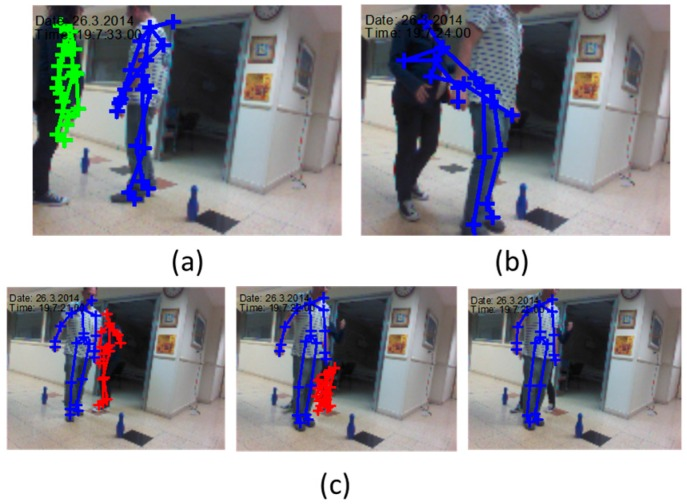
\includegraphics[width=\textwidth]{pictures/sensors-16-01965-g006.jpg}
\caption{Diverse falsch erkannte Skelette.
\begin{enumerate}[label=(\alph*)]
\item degenerierte Skelette
\item verschmolzenes Skelett
\item Skelettverlust durch verdeckung
\end{enumerate}
Quelle: \cite{bodyprop}}
\label{fig:fehlerk}
\end{figure}
\par
	Diese Probleme üben einen negativen Einfluss auf die Erfahrung aus, die der Nutzer mit der Software macht. Insbesondere Fehler nach dem erstgenannten Schema können dem Nutzer das Erreichen seines Zieles -- etwa des Annavigierens eines Objektes -- unmöglich machen. Die weiteren Punkte werden dagegen einfach als störend empfunden. Die verschiedenen (und auch üblichen) von uns angewendeten Mechanismen, um diese Probleme zu beheben, sind weiter unten erklärt.\par
	Die genannten Schwierigkeiten ergeben sich üblichen Problemen von Sensoren wobei hier hinzukommt, dass die Kinect (wegen der primären Anwendung, die die Spieleindustrie zum Ziel hatte) über vergleichsweise preiswerte Sensoren verfügt. In diversen Arbeiten, die sich mit ähnlichen Problemstellungen beschäftigen, finden die Grenzen der Kinect nahezu durchgängig Erwähnung und ein wesentlicher Punkt in der Auseinandersetzung mit der Kinect und ihrer Anwendung in unserem und ähnlichen Szenarien widmet sich einer möglichst fehlerarmen Auswertung der qualitativ durchwachsenen Daten. In der Regel wird dabei auf Verzerrungen und schlechte Werte eingegangen, die sich durch den eingeschränkten \glqq Abdeckbereich\grqq{} der Kinect und den Einfluss von Licht ergeben (siehe \cite{bodyprop} und \cite{kinectlight}). Ferner wird darauf hingewiesen, dass das Detektions- und Trackingproblem generell von Beleuchtung, Blickwinkel, Distanz und weiteren Faktoren abhängt (vgl. \cite{thermalsens}). Ferner ist ein gerade für uns wichtiger Punkt die Abhängigkeit der Kinect-Daten von der Pose, was etwa bereits in \cite{biomid} festgestellt wurde. So ist es beispielsweise möglich, durch ungünstiges Verdecken von Körperpartien die durch die Kinect erkannten Gelenkpositionen zu verschieben. Im Test konnten wir so eine Verschiebung des Genicks (gemeint ist der Gelenkpunkt zwischen Schultern und Hals bzw. Kopf) um mehrere Zentimeter reproduzieren, indem die Hände vor dieser Stelle auf und ab bewegt werden. Besonders kritisch ist dies vor allem dann, wenn die Verdeckung nach dem Verschieben aufgehoben wird und der Gelenkpunkt an seine eigentliche Position \glqq zurückschnappt\grqq{}.
	Der ursprüngliche Ansatz, Pufferung und Mittelung, eliminiert die jitterartigen Fehler, mit denen die Kinectdaten häufig belastet sind. Hierzu wird ein Puffer vorher festgelegter Länge verwendet und während des Programmablaufs mit den für den Anwendungszweck wichtigen Daten, hier den Handpositionen des Nutzers gefüllt. Wenn unser Programm schließlich die Rückgabeparameter für die Manipulationen bestimmt, wird dieser Puffer ausgewertet. Wir bilden dabei ein exponentiell gewichtetes Mittel der gepufferten Positionen. Die neuesten Puffereinträge werden am stärksten gewichtet. Dieser Puffer dient dabei noch gleich einem anderen Zweck: Tests haben ergeben, dass das Steuern angenehmer ist, wenn die Übertragung nicht vollständig direkt von den Handpositionen erfolgt. Die Pufferlänge wurde genau so angelegt, dass das dadurch erzeugte Delay dem Nutzer nicht unangenehm auffällt und gleichzeitig die Kontrolle über das Programm per Gestensteuerung wesentlich glatter und angenehmer erfolgen kann.\par 
	Die eben beschriebene Glättung mag zwar kleine Jitterfehler ausmerzen, versagt jedoch bei Kinectdaten, die sehr stark von den eigentlichen Realdaten abweichen. Ein Beispiel für dieses immer wieder auftauchende Problem ist etwa ein weiterer Nutzer der sich im Hintergrund des steuernden Nutzers bewegt. In einem solchen Fall (und ähnlichen Fällen) kann es passieren, dass die Kinect Körperteile dieses zweiten Nutzers falsch interpretiert und dem Steuernden zuordnet. Dadurch können z.\,B. Positionsdaten entstehen, die um mehrere Meter von der Realtität abweichen. Diese Fehler benötigen eine eigene Ausreißerbehandlung: Werte, die eine zu große Abweichung von den zuletzt ermittelten Werten aufweisen (etwa eine Änderung der Handposition um mehrere Meter in aufeinanderfolgenden Frames) und daher unplausibel sind, werden auf eine vordefinierte Maximalabweichung geclippt. Ohne eine solche Behandlung hätten diese Ausreißer dazu führen können, dass der Nutzer seine aktuelle Position in der 3D-Welt ohne sein Zutun mit großer Geschwindigkeit verlässt (falls er sich etwa im Kamerabewegungsmodus befand).\par 
	Mit den gerade besprochenen Methoden haben wir also eine Reihe von Robustheitsmechanismen, was fehlerhafte Kinectdaten hinsichtlich der Position von Joints (Gelenkpunkten) angeht. Dies ist nicht der einzige Aspekt der Anwendung, der solche Sonderbehandlungen verlangt. Wir hatten oben bereits als einen derartigen Punkt die Erkennung der \glqq Hand States\grqq{} genannt. Hier ist insbesondere kritisch, dass eine Fehlerkennung nach dem ursprünglichen Modell, das nur Handzustände zu einem bestimmten Zeitpunkt diskret ausgewertet hat, zu sofortigen Zustandswechseln der Zustandsmaschine führen konnte. Besonders häufig erkennt die Kinect Handzustände in den Fehlersituationen gar nicht (und drückt dies durch \glqq Erkennen\grqq{}) des Zustands \glqq{}Unknown\grqq{} aus), teils -- wenn auch deutlich seltener -- werden jedoch auch die \glqq echten\grqq{} Zustände \glqq offen\grqq{}, \glqq geschlossen\grqq{} und \glqq Lasso\grqq{} falsch zugeordnet.\par 
	Wir wollen ferner Folgendes bemerken: Obwohl die Kinect (auch nicht intern) über keine eigenen Identifikationsmechanismen verfügt (vgl. \cite{bodyprop}), legt die durch das im SDK enthaltene Kinect Studio (siehe \cite{kinectsdk}) nahe, dass wenigstens von der Kinect mitgelieferte Konfidenzwerte für die Güte der Rückgabedaten verfügbar sind. Diese Überlegung drängte sich auf, da schlecht erkannte Gelenke (bzw. eher Gelenkverbindungen) im Studio dünner dargestellt werden, als jene, bei denen die Kinect-Daten gut zu sein scheinen: Dünne Verbindungen treten überwiegend bei Verdeckung und am Sichtfensterrand auf. Es stellte sich jedoch heraus, dass alles, was die Kinect in dieser Hinsicht bereitstellt aus drei Status pro Gelenkpunkt besteht: Jeder Gelenkpunkt ist getrackt (\glqq Tracked\grqq), nicht getrackt (\glqq NotTracked\grqq) und vermutet (\glqq Inferred\grqq). Über den letzten Status ist der Dokumentation (siehe \cite{trackingstate}) nur zu entnehmen, dass das Vertrauen in die Richtigkeit der Daten \glqq sehr gering\grqq{} ist.
